\documentclass[border=3pt]{standalone}
% Preâmbulo compartilhado pelos diagramas TikZ da aula 9 de IHR (Robôs na Sociedade)
\usepackage[T1]{fontenc}
\usepackage[utf8]{inputenc}
\usepackage{lmodern}
\usepackage{amsmath}
\usepackage{xcolor}
\usepackage{tikz}
\usetikzlibrary{arrows.meta,angles,quotes,decorations.pathmorphing,decorations.pathreplacing,calc,
                positioning,shapes.geometric,shapes.misc,backgrounds,fit,
                math}

% Paleta (mesma dos SVGs originais)
% Paleta da disciplina de IHR: acento azul (#1A6FB5), cor de destaque do tema.
% (o nome "dblue" é mantido para não alterar todos os diagramas)
\definecolor{dblue}{HTML}{1A6FB5}
\definecolor{dorange}{HTML}{B3541E}
\definecolor{dgreen}{HTML}{4A7C59}
\definecolor{dred}{HTML}{9C4B4B}
\definecolor{dcream}{HTML}{F4F1EA}
\definecolor{dshade}{HTML}{DDD7C9}

% Função gaussiana (não normalizada por padrão de escala visual)
\pgfmathdeclarefunction{gauss}{3}{%
  \pgfmathparse{1/(#3*sqrt(2*pi))*exp(-((#1-#2)^2)/(2*#3^2))}%
}

% Estilos comuns (prefixo d... para não colidir com chaves internas do pgf)
\tikzset{
  >={Stealth[length=2mm]},
  dguide/.style={gray!55, dashed, line width=0.4pt},
  daxis/.style={gray!60, line width=0.7pt, ->},
  dbody/.style={fill=black!3, draw=black!80, line width=1pt},
  dacc/.style={draw=dblue, line width=1pt},
  dlbl/.style={black!55, font=\small},
  dsub/.style={black!45, font=\footnotesize},
  dstate/.style={circle, draw=black!80, fill=dcream, line width=1pt,
                 minimum size=17mm, font=\large, inner sep=1pt},
  dobs/.style={circle, draw=black!80, fill=dshade, line width=1pt,
               minimum size=14mm, font=\large, inner sep=1pt},
  dbox/.style={rounded corners=2pt, draw=black!80, fill=dcream, line width=1pt,
               align=center, inner sep=6pt},
  dop/.style={circle, draw=black!80, fill=white, line width=1pt,
              minimum size=6mm, inner sep=0pt, font=\small},
  dtrans/.style={->, dblue, line width=1pt},
  dmeas/.style={->, dorange, line width=1pt},
  dcurve/.style={line width=1pt, dblue},
  dcurveb/.style={line width=1.4pt, dorange},
}

\begin{document}
\hyphenpenalty=10000 \exhyphenpenalty=10000 \tolerance=9999 \emergencystretch=3em
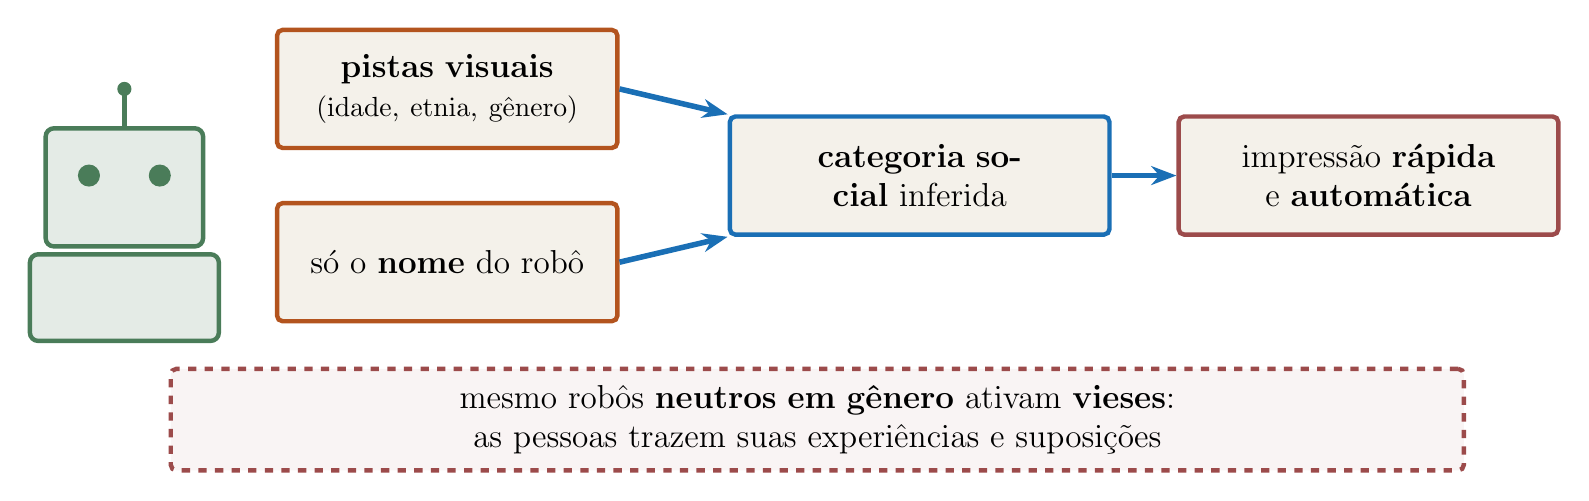
\begin{tikzpicture}[x=1cm,y=1cm]
\tikzset{k/.style={dbox, text width=4.6cm, minimum height=1.5cm, font=\large, line width=1.6pt}}
% robo
\draw[dgreen, fill=dgreen!15, line width=1.6pt, rounded corners=3pt] (0.2,2.4) rectangle (2.2,3.9);
\fill[dgreen] (0.75,3.3) circle (0.14); \fill[dgreen] (1.65,3.3) circle (0.14);
\draw[dgreen, line width=1.6pt] (1.2,3.9) -- (1.2,4.35); \fill[dgreen] (1.2,4.4) circle (0.09);
\draw[dgreen, fill=dgreen!15, line width=1.6pt, rounded corners=3pt] (0.0,1.2) rectangle (2.4,2.3);
\node[k, draw=dorange, text width=3.9cm] (a) at (5.3,4.4) {\textbf{pistas visuais}\\ {\normalsize (idade, etnia, gênero)}};
\node[k, draw=dorange, text width=3.9cm] (b) at (5.3,2.2) {só o \textbf{nome} do robô};
\node[k, draw=dblue, text width=4.4cm] (c) at (11.3,3.3) {\textbf{categoria social} inferida};
\node[k, draw=dred, text width=4.4cm] (d) at (17.0,3.3) {impressão \textbf{rápida} e \textbf{automática}};
\draw[dtrans, line width=2pt, -{Stealth[length=3.2mm]}] (a.east) -- (c.north west);
\draw[dtrans, line width=2pt, -{Stealth[length=3.2mm]}] (b.east) -- (c.south west);
\draw[dtrans, line width=2pt, -{Stealth[length=3.2mm]}] (c.east) -- (d.west);
\node[dbox, draw=dred, dashed, fill=dred!6, line width=1.6pt, text width=16cm, minimum height=1.2cm, font=\large] at (10.0,0.2) {mesmo robôs \textbf{neutros em gênero} ativam \textbf{vieses}: as pessoas trazem suas experiências e suposições};
\end{tikzpicture}
\end{document}
